

\documentclass[10pt]{beamer}

\mode<presentation>
{
 \usetheme{Boadilla}
\pagestyle{empty}

\setbeamerfont*{frametitle}{size=\normalsize,series=\bfseries}
\setbeamerfont*{block}{size=\normalsize,series=\bfseries}
%\setbeamertemplate{blocks}[rounded][shadow=true]
}

\definecolor{links}{HTML}{2A1B81}
\hypersetup{colorlinks,linkcolor=,urlcolor=links}


\usepackage[pdf]{pstricks}
\usepackage{pst-sigsys}


\definecolor{darkblue}{rgb}{0.0, 0.0, 0.40}
\setbeamercolor{title}{fg=darkblue}
\setbeamercolor{frametitle}{fg=darkblue}
\definecolor{darkgreen}{rgb}{0.0, 0.4, 0.0}

\usepackage{bbm}


\def\nn{\nonumber}
\def\xt{x(t)}
\def\xn{x[n]}
\def\xeven{x_{\text{even}}}
\def\xodd{x_{\text{odd}}}

\newcommand{\fs}[2]{#2}

\title[]{Periodicity, Energy and Power}
\author[\textcolor{blue}{Systems and Circuits}]{\textcolor{darkblue}{Pablo M. Olmos} (olmos@tsc.uc3m.es)\\ \textcolor{darkblue}{Emilio Parrado} (emipar@tsc.uc3m.es)}
\institute{\textcolor{white}{UC3M}}


\AtBeginSection[]
{
  \begin{frame}<beamer>{Index}
    \tableofcontents[currentsection,currentsubsection]
  \end{frame}
}






%%%%%%%%%%%%%%%%
\begin{document}

\frame{
\titlepage
\thispagestyle{empty}
\begin{center}

\includegraphics[scale=0.05]{Figures/uc3m-logo2.pdf}
\end{center}
}

\section{Properties of signals}

\subsection{Symmetry}

\frame{
\frametitle{Even and odd signals}

\begin{exampleblock}{Even signal}
$\xt$ presents even symmetry (shortly, it is an even signal) if:
\begin{align}\nn
\xt=x(-t) \qquad \forall t
\end{align} 
The same definition holds for sequences: $\xn$ is even if $\xn=x[-n]$ $\forall n$.
\end{exampleblock}

By definition, an even signal is symmetric with respect to the coordinate axis.

}


\frame{

\begin{figure}
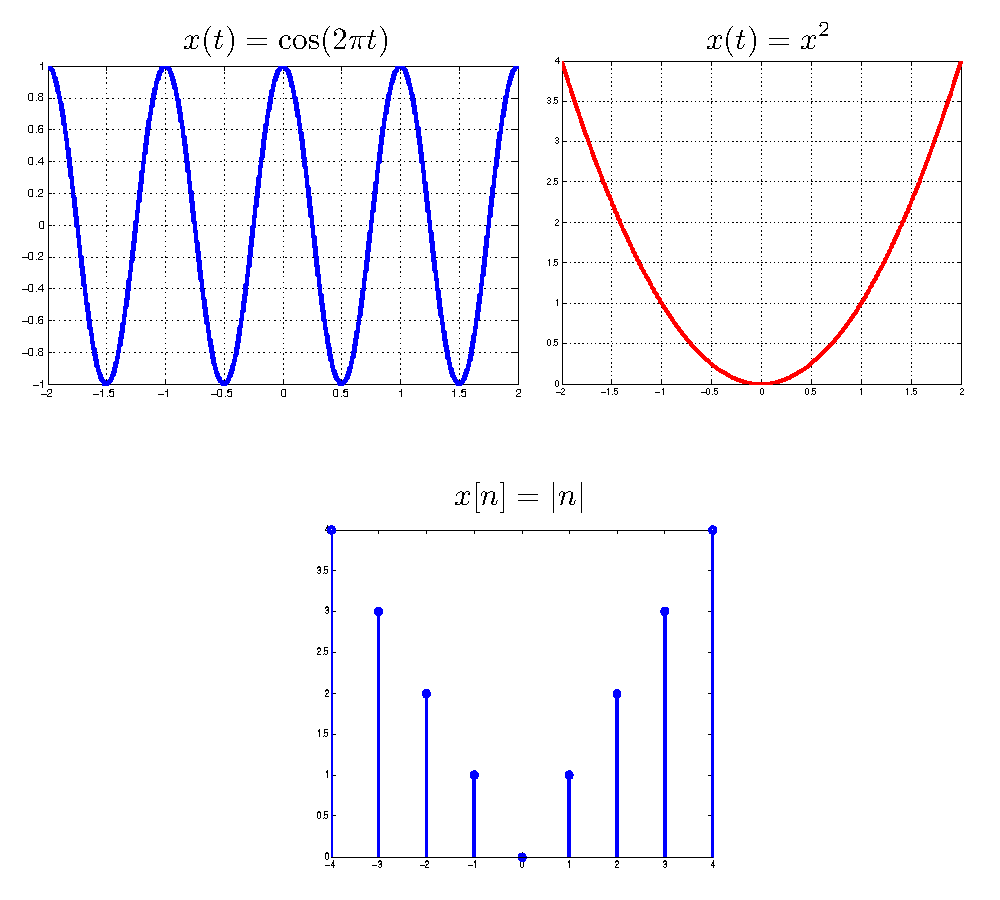
\includegraphics[scale=0.6]{Figures/Signal29.pdf}
\end{figure}

}

\frame{

\begin{exampleblock}{Odd signal}
$\xt$ presents odd symmetry (shortly, it is an odd signal) if:
\begin{align}\nn
\xt=-x(-t) \qquad \forall t
\end{align} 
The same definition holds for sequences: $\xn$ is odd if $\xn=-x[-n]$ $\forall n$.
\end{exampleblock}

\begin{alertblock}{}
Necessarily, if $\xt$ ($\xn$) is odd, then $x(0)=0$ ($x[0]=0$)!!! 
\end{alertblock}

}


\frame{

\begin{figure}
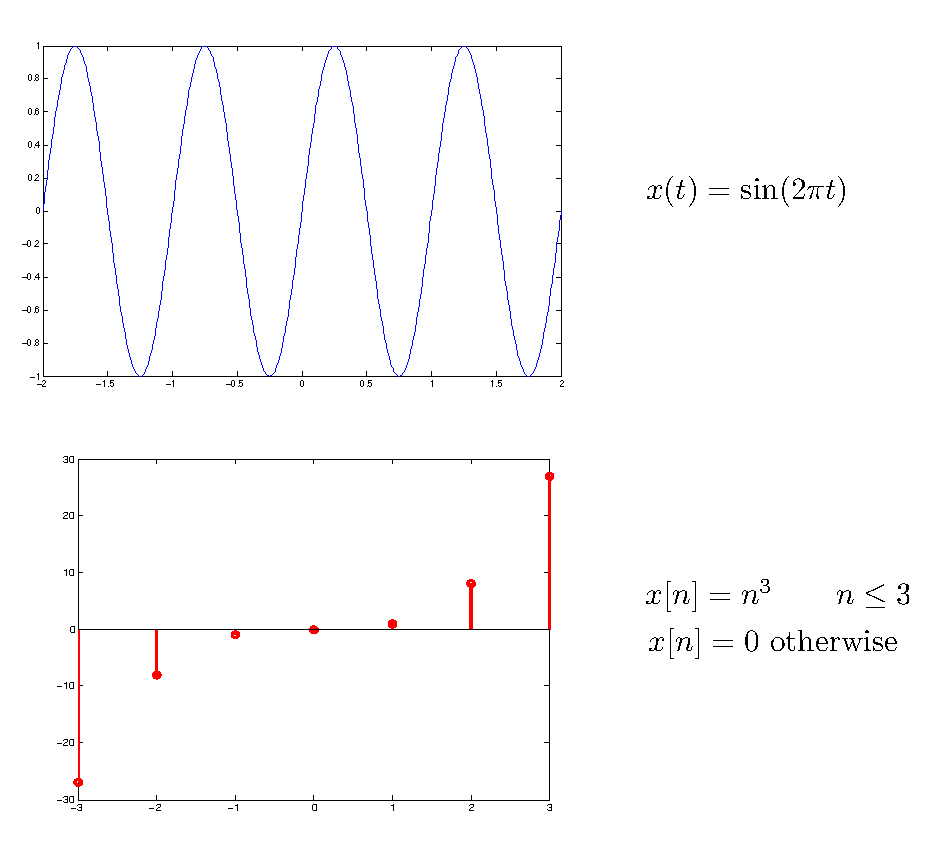
\includegraphics[scale=0.6]{Figures/Signal_32.pdf}
\end{figure}

}

\frame{
\frametitle{Even and Odd parts of a signal}
\begin{block}{}
Any signal $x(t)$ can be decomposed as the sum of an even signal $\xeven(t)$ plus an odd signal $\xodd(t)$:
\begin{align}\nn
x(t)=\xeven(t)+\xodd(t)\\\nn
x[n]=\xeven[n]+\xodd[n]
\end{align}
\end{block}

\begin{alertblock}{}
$\xeven$ and $\xodd$ are simply computed as follows:
\begin{align}\nn
&\xeven(t)=\frac{x(t)+x(-t)}{2}\qquad \xeven[n]=\frac{x[n]+x[-n]}{2}\\\nn
&\xodd(t)=\frac{x(t)-x(-t)}{2}\qquad \;\;\xodd[n]=\frac{x[n]-x[-n]}{2}
\end{align}
\end{alertblock}

}

\frame{

\begin{figure}
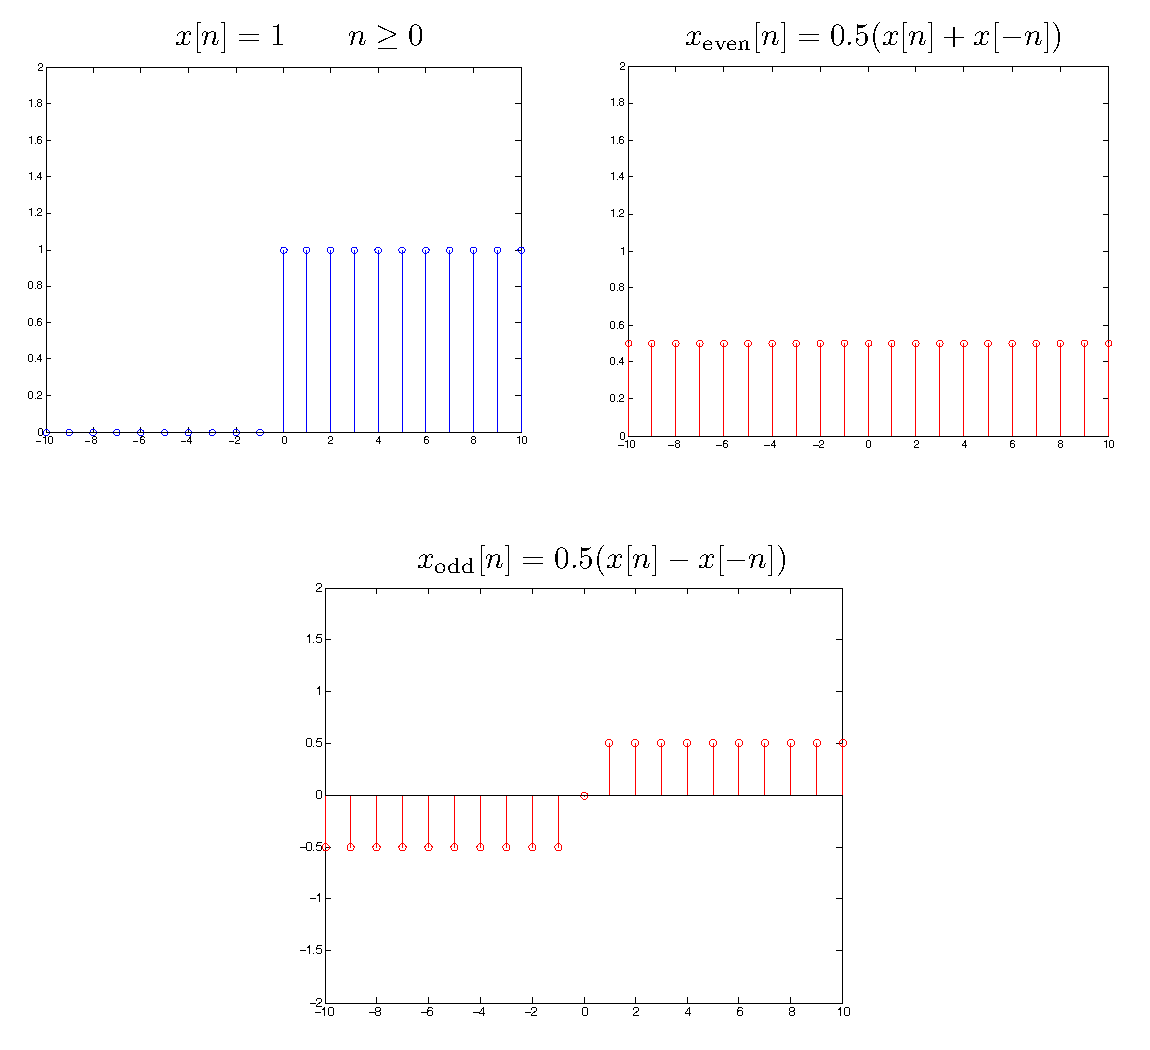
\includegraphics[scale=0.5]{Figures/Signal_36.pdf}
\end{figure}

}

\subsection{Periodicity}

\frame{
\frametitle{Periodic continuous signals}

\begin{block}{}
$x(t)$ is periodic if there exists a real number $T$ such that $x(t)=x(t+T)$ for any $t$. 
\end{block}

\begin{exampleblock}{$\cos(\frac{2}{3}\pi t)$}
\begin{align}\nn
&\cos(\frac{2}{3}\pi (t+T))=\cos(\frac{2}{3}\pi t) \Leftrightarrow \frac{2}{3}\pi T=2\pi k\quad k\in\mathbb{Z}\\\nn
&\Rightarrow T=3k\qquad k=1,2,3,\ldots
\end{align}
\textbf{$T=3$ is the \color{red}{fundamental period.}}
\end{exampleblock}

}

\frame{
Given $x(t)=\cos(2\pi t)+\sin (\frac{\pi}{3}t)$:
\begin{itemize}
\item Is $x(t)$ periodic?
\item What is the fundamental period?
\end{itemize}

%\textbf{Sol.:}
%
%\begin{enumerate}
%\item $\cos(2\pi t)$ is periodic with period $T_1=k$ for $k=1,2,\ldots$
%\item $\sin (\frac{\pi}{3}t)$ is periodic with period $T_2=6k$ for $k=1,2,\ldots$
%\item Least common multiple: $6k$.
%\item Thus $x(t)$ is periodic with period $T=6k$ and fundamental period $T=6$.
%\end{enumerate}

}

\frame{
\frametitle{Example}
Given $x(t)=\cos(2\pi t)+\sin (\frac{\pi}{3}t)$:
\begin{itemize}
\item Is $x(t)$ periodic?
\item What is the fundamental period?
\end{itemize}

\textbf{Sol.:}

\begin{enumerate}
\item $\cos(2\pi t)$ is periodic with period $T_1=k$ for $k=1,2,\ldots$
\item $\sin (\frac{\pi}{3}t)$ is periodic with period $T_2=6k$ for $k=1,2,\ldots$
\item Least common multiple: $6k$.
\item Thus $x(t)$ is periodic with period $T=6k$ and fundamental period $T=6$.
\end{enumerate}

}

\frame{

$x(t)=\cos(2\pi t)+\sin (\frac{\pi}{3}t)$
\begin{figure}
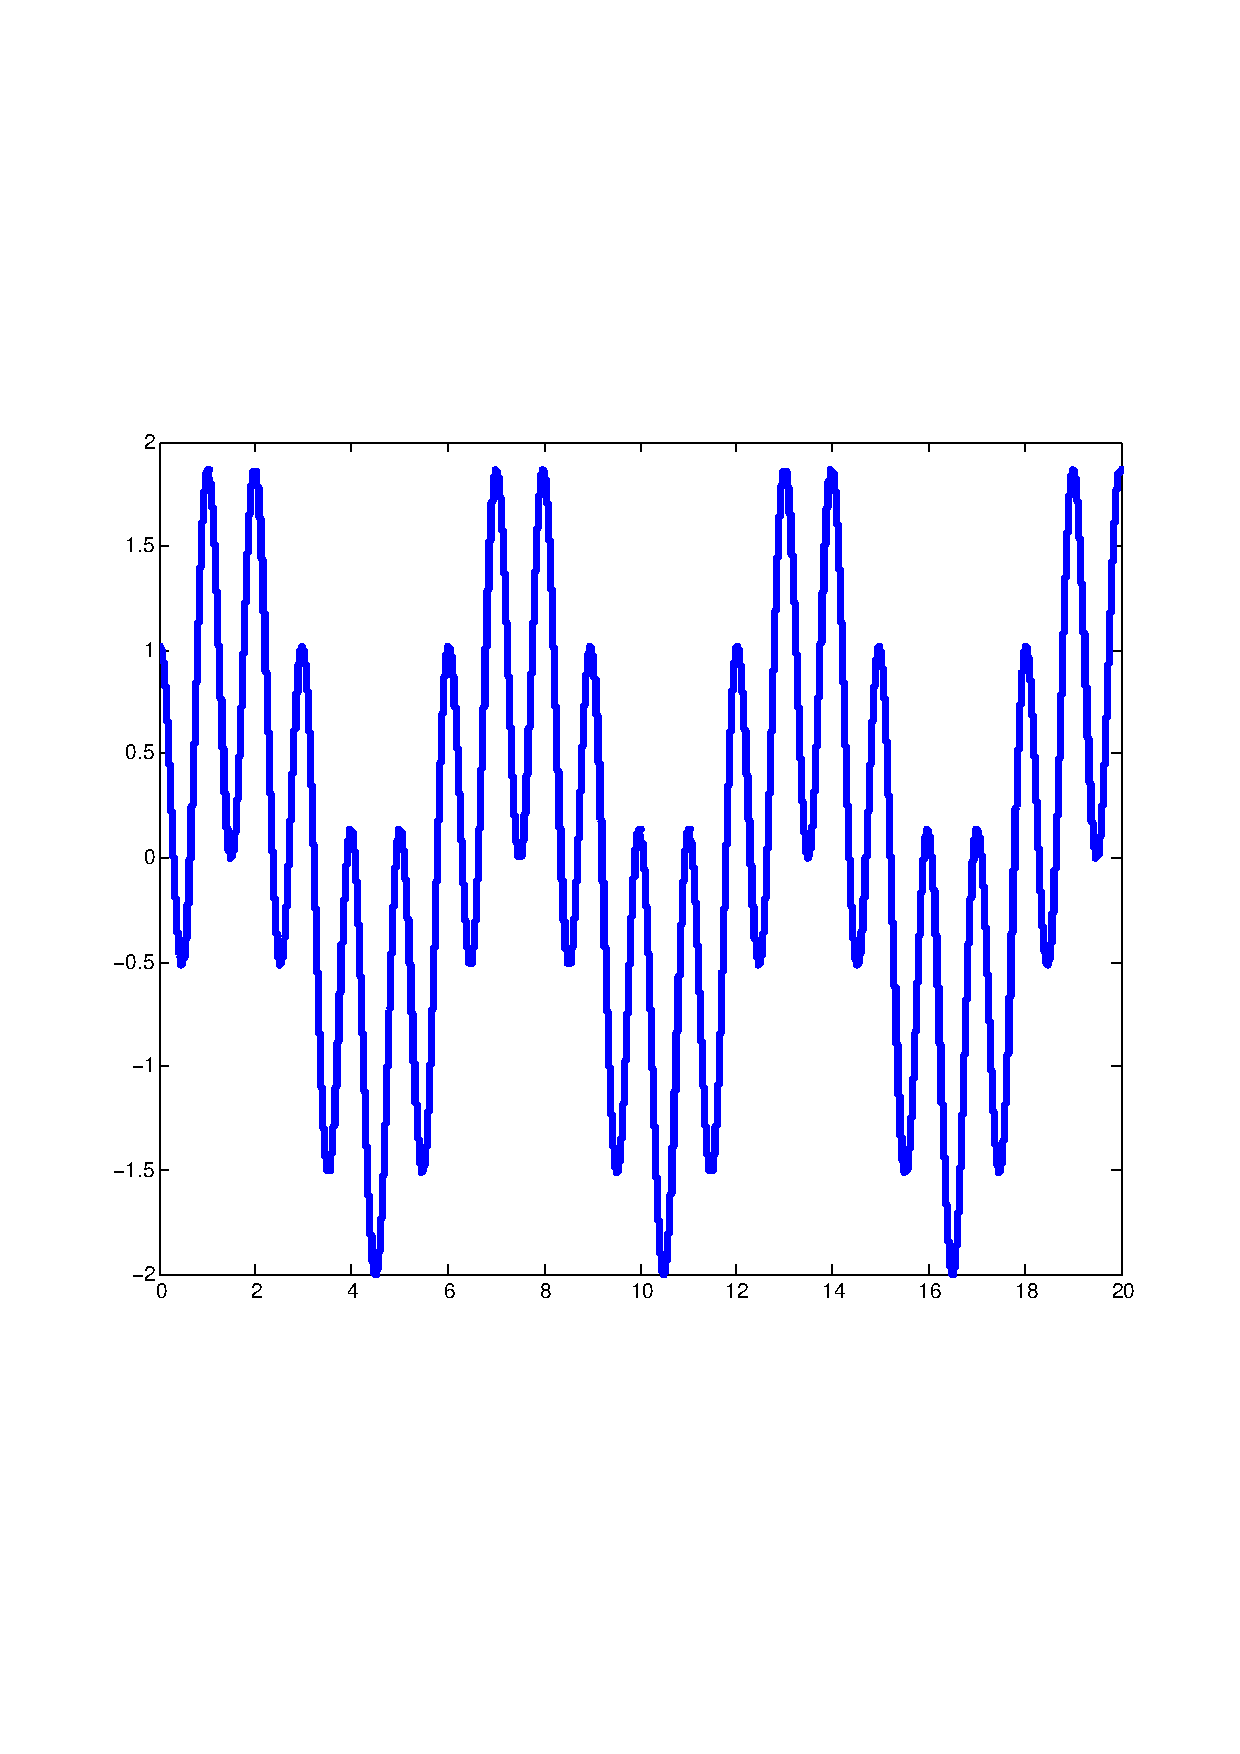
\includegraphics[scale=0.3]{Figures/Signal35.pdf}
\end{figure}

}


\frame{
\frametitle{Periodic sequences}

\begin{block}{}
$x[n]$ is periodic if there exists an integer number $N$ such that $x[n]=x[n+N]$ for any $n$. 
\end{block}

\begin{exampleblock}{$\cos(\frac{1}{7}\pi n)$}
\begin{align}\nn
&\cos(\frac{1}{7}\pi (n+N))=\cos(\frac{1}{7}\pi n) \Leftrightarrow \frac{1}{7}\pi N=2\pi k\quad k\in\mathbb{Z}\\\nn
&\Rightarrow N=14k\qquad k=1,2,3,\ldots
\end{align}
\textbf{$N=14$ is the \color{red}{fundamental period.}}
\end{exampleblock}

}

\frame{

\begin{alertblock}{$\cos(\frac{1}{7} n)$}
\begin{align}\nn
&\cos(\frac{1}{7} (n+N))=\cos(\frac{1}{7} n) \Leftrightarrow \frac{1}{7} N=2\pi k\quad k\in\mathbb{Z}\\\nn
&\color{red}{\Rightarrow N=14\pi k\qquad k=1,2,3,\ldots \text{ Never an integer!!}}
\end{align}
\textbf{$\cos(\frac{1}{7} n)$ is not periodic!! Though it may look as periodic...}
\end{alertblock}

\begin{figure}
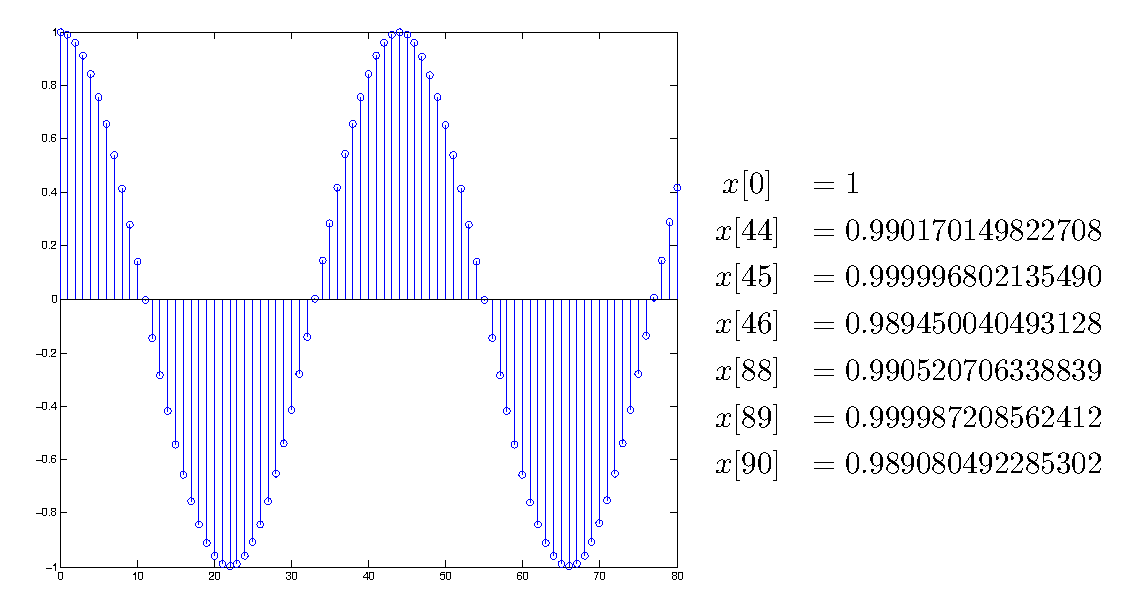
\includegraphics[scale=0.5]{Figures/Signal41.pdf}
\end{figure}


}


\subsection{Average value}

\frame{
\frametitle{Signal average value}

\begin{block}{Average value over a given interval (partial average)}
\begin{align}\nn
<x(t)>_{t_a,t_a+L}=\frac{1}{L}\int_{t_a}^{t_a+L}x(t) dt\\\nn
<x[n]>_{n_a,n_a+I}=\frac{1}{I+1}\sum_{n_a}^{n_a+I}x[n]
\end{align}
\end{block}

%\begin{alertblock}{}
%$T_0$ and $N_0$ are just the interval lengths!
%\end{alertblock}

}


\frame{
\begin{figure}
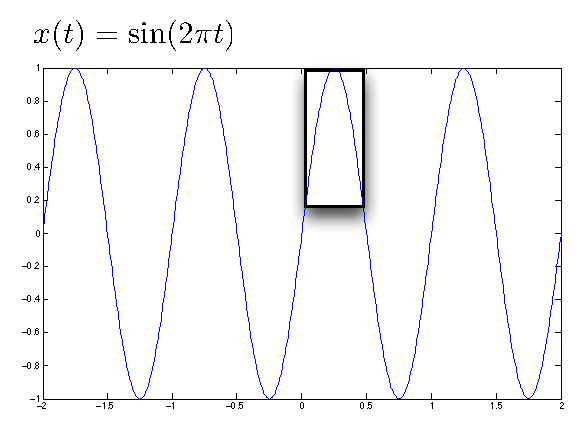
\includegraphics[scale=0.7]{Figures/Signal_21.pdf}
\end{figure}
\begin{align}\nn
<x(t)>_{0,\frac{1}{2}}=\frac{1}{1/2}\int_0^{1/2}\sin(2\pi t) dt=-\frac{1}{\pi}[\cos(2\pi t)]_0^{1/2}=\frac{2}{\pi}
\end{align}

}

\frame{
\begin{figure}
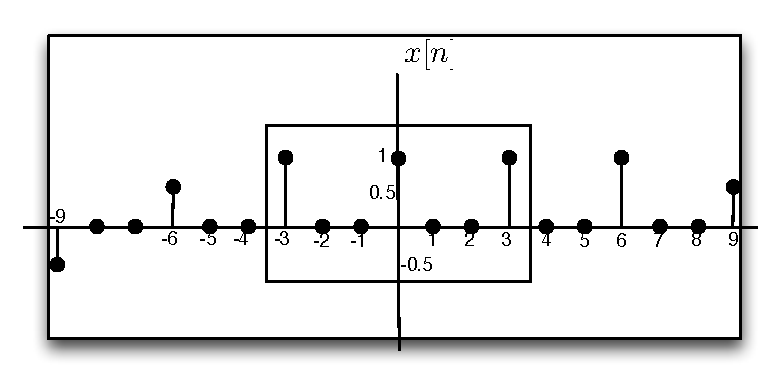
\includegraphics[scale=0.7]{Figures/Signal_22.pdf}
\end{figure}
\begin{align}\nn
&<x[n]>_{-3,3}=\frac{3}{7}\\\nn
&<x[n]>_{-9,9}=\frac{4.5}{19}
\end{align}

}

\frame{

\begin{block}{Average value}
\begin{align}\nn
<x(t)>=\lim_{L\rightarrow\infty} \frac{1}{2L}\int_{-L}^{L}x(t) dt\\\nn
<x[n]>=\lim_{I\rightarrow\infty} \frac{1}{2I+1}\sum_{-I}^{I}x[n]
\end{align}
\end{block}

%\begin{exampleblock}{}
%If the signal $x(t)$ is defined only for $t\in[a,b]$, by average value we mean the partial average value computed across $[a,b]$.
%\end{exampleblock}

}

\frame{
\begin{figure}
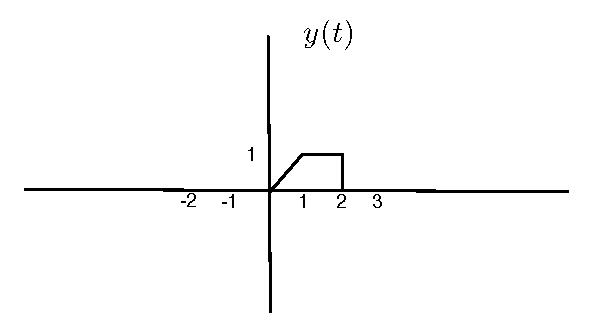
\includegraphics[scale=0.7]{Figures/Signal_26.pdf}
\end{figure}

\begin{align*}
<x(t)>&=?\\
<x(t)>&_{0,2}=?
\end{align*}
}

\frame{
\begin{figure}
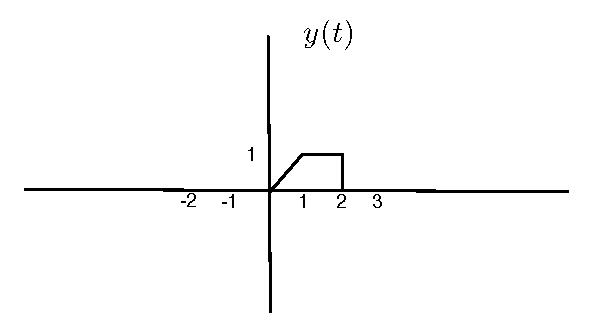
\includegraphics[scale=0.7]{Figures/Signal_26.pdf}
\end{figure}

\begin{align*}
<x(t)>&=\lim_{L\rightarrow\infty} \frac{1}{2L}\int_{-L}^{L}x(t) dt=\lim_{L\rightarrow\infty} \frac{1}{2L}\int_{0}^{2}y(t)dt\\&=\lim_{L\rightarrow\infty} \frac{1}{2L} \left[\int_{0}^{1}tdt+\int_{1}^{2}1dt \right]=\lim_{L\rightarrow\infty}\frac{1}{2L}\left(\frac{1}{2}+1\right)=0\\
\color{red}{}<x(t)>&_{\color{red}{}0,2}\color{red}{}=3/4
\end{align*}
}


\frame{
\begin{figure}
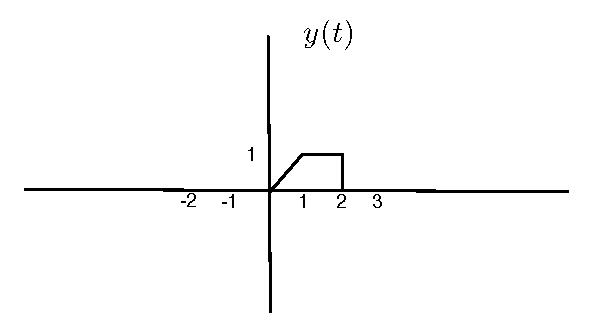
\includegraphics[scale=0.7]{Figures/Signal_26.pdf}
\end{figure}

\begin{align*}
<x(t)>&=\lim_{L\rightarrow\infty} \frac{1}{2L}\int_{-L}^{L}x(t) dt=\lim_{L\rightarrow\infty} \frac{1}{2L}\int_{0}^{2}y(t)dt\\&=\lim_{L\rightarrow\infty} \frac{1}{2L} \left[\int_{0}^{1}tdt+\int_{1}^{2}1dt \right]=\lim_{L\rightarrow\infty}\frac{1}{2L}\left(\frac{1}{2}+1\right)=0\\
\color{red}{}<x(t)>&_{\color{red}{}0,2}\color{red}{}=3/4
\end{align*}
}


\frame{
\begin{alertblock}{Average value: Periodic signals}
If $x(t)$ is periodic with fundamental period $T$, then for any $t_0\in\mathbb{R}$
\begin{align}\nn
<x(t)>= \frac{1}{T}\int_{t_0-\frac{T}{2}}^{t_0+\frac{T}{2}}x(t) dt
\end{align}
\end{alertblock}
\begin{alertblock}{Average value: Periodic signals}
If $x[n]$ is periodic with fundamental period $N$, then for any $n_0\in\mathbb{Z}$
\begin{align}\nn
<x[n]>=\frac{1}{N}\sum_{n_0}^{n_0+N-1}x[n]
\end{align}
\end{alertblock}
}

\frame{
\begin{figure}
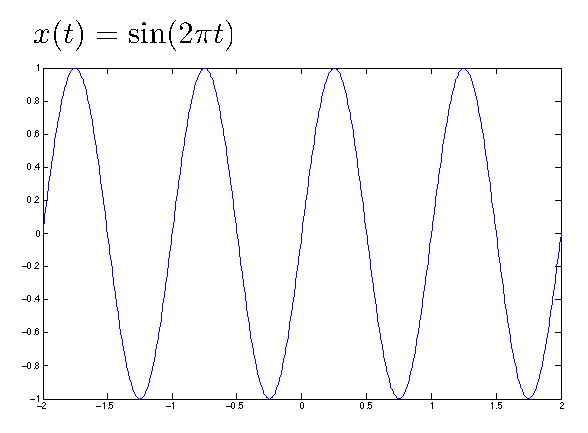
\includegraphics[scale=0.7]{Figures/Signal_24.pdf}
\end{figure}
\begin{align}\nn
<x(t)>=\int_0^{1}\sin(2\pi t) dt=-\frac{1}{2\pi}[\cos(2\pi t)]_0^{1}=0
\end{align}

}


\subsection{Power and Energy}

\frame{
\frametitle{Signal Power}

Assume $x(t)$ is a voltage signal in an electric circuit.
\begin{figure}
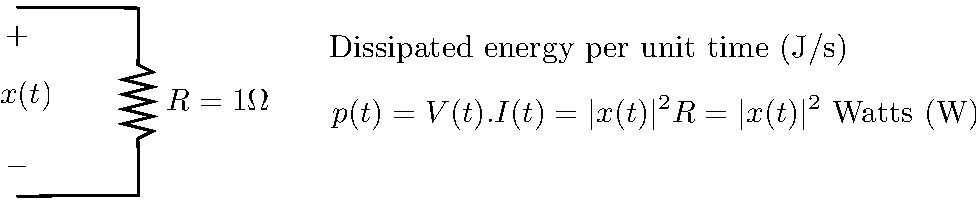
\includegraphics[scale=0.7]{Figures/Signal_25.pdf}
\end{figure}

\begin{exampleblock}{}
$p_x(t)=|x(t)|^{2}$ is defined as the power signal associated to $x(t)$ (\textbf{It is a signal}!!).
\end{exampleblock}

\begin{exampleblock}{}
The same definition holds for sequences. $p_x[n]=|x[n]|^2$ is the power signal associated to $x[n]$.
\end{exampleblock}

}

\frame{
\frametitle{Average signal power}


\begin{block}{Average signal power in a given interval}
\begin{align}\nn
<p_x(t)>_{t_a,t_a+L}=\frac{1}{L}\int_{t_a}^{t_a+L}|x(t)|^{2} dt\quad \text{W}\\\nn
<p_x[n]>_{n_a,I}=\frac{1}{I+1}\sum_{n_a}^{n_a+I}|x[n]|^{2}  \quad \text{W}
\end{align}
\end{block}

\begin{block}{Average power}
\begin{align}\nn
P_x=\lim_{L\rightarrow\infty} \frac{1}{2L}\int_{-L}^{L}|x(t)|^{2} dt \quad \text{W}\\\nn
P_x=\lim_{I\rightarrow\infty} \frac{1}{2I+1}\sum_{-I}^{I}|x[n]|^{2} \quad \text{W}
\end{align}
\end{block}

}

\frame{

\frametitle{Average power: periodic signals}

If $x(t)$ (or $x[n]$) is periodic with fundamental period $T$, then $p_x(t)$ ($p_x[n]$) is also periodic and $T$ is a valid period. Thus,

\begin{alertblock}{Average Power: Periodic signals}
If $x(t)$ is periodic with fundamental period $T$, then for any $t_0\in\mathbb{R}$
\begin{align}\nn
P_x= \frac{1}{T}\int_{t_0-\frac{T}{2}}^{t_0+\frac{T}{2}}|x(t)|^{2} dt \quad \text{W}
\end{align}
\end{alertblock}

\begin{alertblock}{Average value: Periodic signals}
If $x[n]$ is periodic with fundamental period $N$, then for any $n_0\in\mathbb{Z}$
\begin{align}\nn
P_x=\frac{1}{N}\sum_{no}^{n_0+N-1}|x[n]|^{2} \quad \text{W}
\end{align}
\end{alertblock}


}

\frame{
\begin{figure}
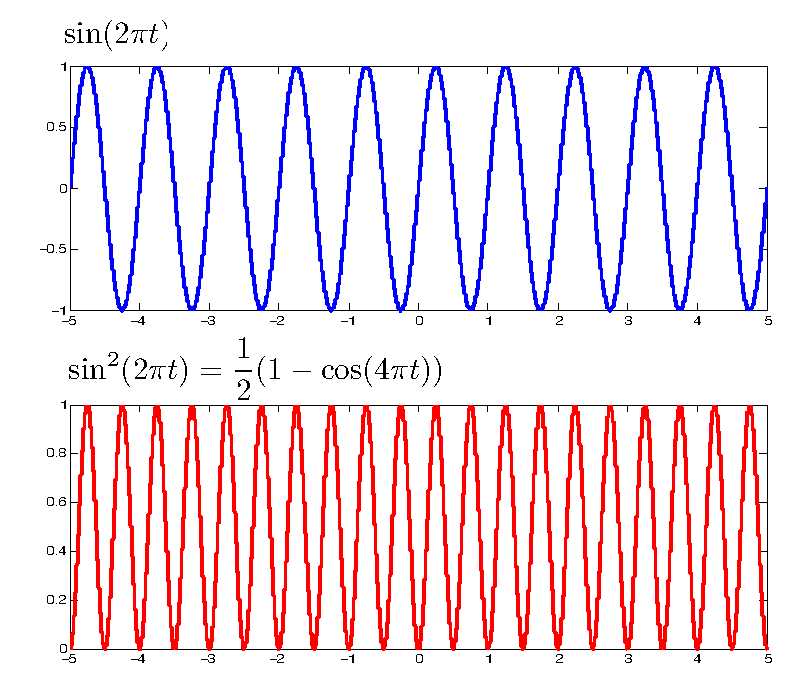
\includegraphics[scale=0.5]{Figures/Signal55.pdf}
\end{figure}

\begin{exampleblock}{}
$\sin(2\pi t)$ has fundamental period $T=1$ s. $\sin^{2}(2\pi t)$ has fundamental period $T=0.5$ s but $T=1$ is a valid period.
\end{exampleblock}
}


\frame{
\begin{figure}
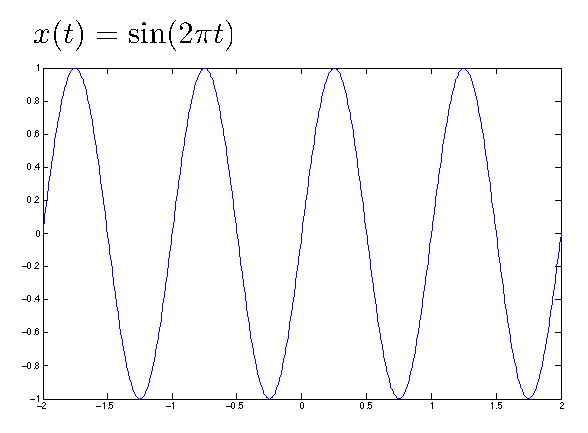
\includegraphics[scale=0.7]{Figures/Signal_24.pdf}
\end{figure}
\begin{align}\nn
P_x=\int_0^{1}\sin^2(2\pi t) dt=\frac{1}{2}\int_0^{1} (1-\cos(4\pi t)) dt=\frac{1}{2} \quad \text{W}
\end{align}

\url{http://www.mathwords.com/t/trig_identities.htm}

%\begin{alertblock}{Trigonometric identities}
%You have to remember them! $\sin(a)\cos(b)$, $\sin(a+b)$, $\cos(a+b)$, $\sin^2(a)$, $\sin^2(b)$, etc...
%\end{alertblock}
}

\frame{
\frametitle{Signal energy}

Given $x(t)$, its energy measured over an interval $[t_a,t_b]$ is the integral of the power signal $p_x(t)$:

\begin{align}\nn
E_x(t_a,t_b)=\int_{t_a}^{t_b}|x(t)|^{2}dt \quad \text{J (joules)}
\end{align}

For sequences,

\begin{align}\nn
E_x[n_a,n_b]=\sum_{n_a}^{n_b}|x[n]|^{2} \quad \text{J}
\end{align}

The total energy of a signal is defined as

\begin{align}\nn
E_x=\int_{-\infty}^{\infty}|x(t)|^{2}dt\qquad E_x=\sum_{-\infty}^{\infty}|x[n]|^{2} \quad \text{J}
\end{align}

}

\frame{

\begin{figure}
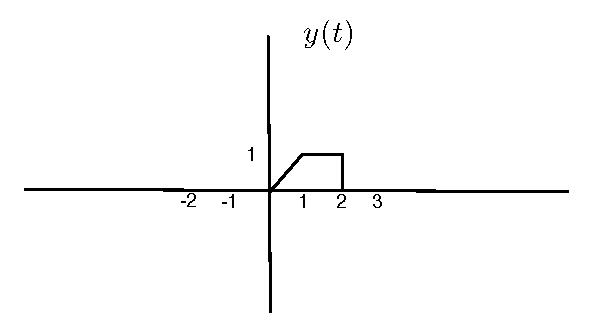
\includegraphics[scale=0.7]{Figures/Signal_26.pdf}
\end{figure}

\begin{align}\nn
E_y=\int_{0}^{1} t^2 dt+\int_{1}^{2} 1 dt =\frac{1}{3} [t^3]_{0}^{1}+1=\frac{4}{3} \quad \text{J} 
\end{align}

}

\frame{
\frametitle{Energy signals and Power signals}
Given $x(t)$,

\begin{itemize}
\item If $E_x< \infty$, then $x(t)$ is an energy signal (or a signal defined in terms of energy)
\item If $E_x\rightarrow \infty$, then $x(t)$ is NOT an energy signal. Besides, if $P_x< \infty$, then $x(t)$ is a power signal (or a signal defined in terms of power).
\item If $P_x\rightarrow \infty$, then is neither an energy signal nor a power signal.
\end{itemize}

}
%
%
%\section{Unit step and impulse}
%
%
%\frame{
%\begin{exampleblock}{In the rest of this class and next Wednesday}
%We describe a set of  basic signal models whose properties are extremely important to analyze and design complex signal processing systems.
%\end{exampleblock}
%
%\begin{figure}
%
\includegraphics[scale=0.2]{Figures/Signal70.pdf}
%\end{figure}
%
%}
%
%\subsection{Discrete-time Unit Impulse and Unit Step}
%
%
%\frame{
%\frametitle{Unit Impulse Sequence (Kronecker delta)}
%
%Probably the simplest sequence we can imagine:
%\begin{align}\nn
%\delta[n]=\left\{
%\begin{array}{cc}
%1 & n=0\\
%0 & n\neq 0
%\end{array}
%\right.
%\qquad
%\delta[n-n_0]=\left\{
%\begin{array}{cc}
%1 & n=n_0\\
%0 & n\neq n_0
%\end{array}
%\right.
%\end{align}
%
%
%\begin{figure}
%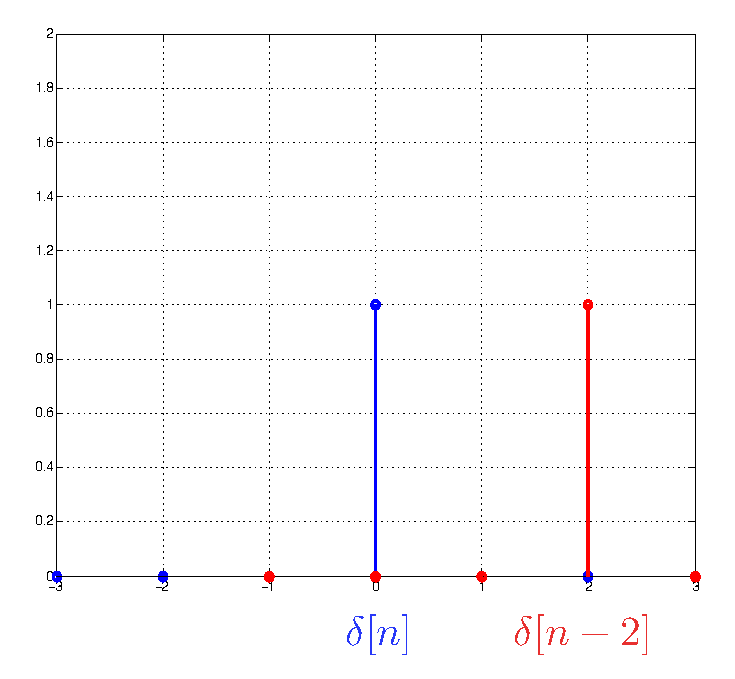
\includegraphics[scale=0.45]{Figures/Signal62.pdf}
%\end{figure}
%
%}
%
%\frame{
%\frametitle{Unit Impulse Sequence. Properties}
%\begin{block}{}
%It is an even signal: $\delta[n]=\delta[-n]$.
%\end{block}
%\begin{alertblock}{}
% Is $\delta[n-n_0]$ an even signal?
%\end{alertblock}
%\begin{exampleblock}{}
%\begin{align}\nn
%x[n]\delta[n-n_0]=\left\{
%\begin{array}{cc}
%x[n_0] & n=n_0\\
%0 & n\neq n_0
%\end{array}
%\right.
%\end{align}
%\end{exampleblock}
%
%\begin{block}{}
%\begin{align}\nn
%\sum_{n=-\infty}^{\infty}\delta[n]=1
%\end{align}
%\end{block}
%
%\begin{exampleblock}{}
%$\delta[n]$ is a signal of finite energy.
%\end{exampleblock}
%
%}
%
%\frame{
%\frametitle{Unit Impulse Sequence. Properties}
%
%\begin{block}{}
%Any signal can be decomposed as a sum of unit impulse sequences:
%\begin{align}\nn
%x[n]=\sum_{k=-\infty}^{\infty}x[k]\delta[n-k]
%\end{align}
%\end{block}
%
%\begin{figure}
%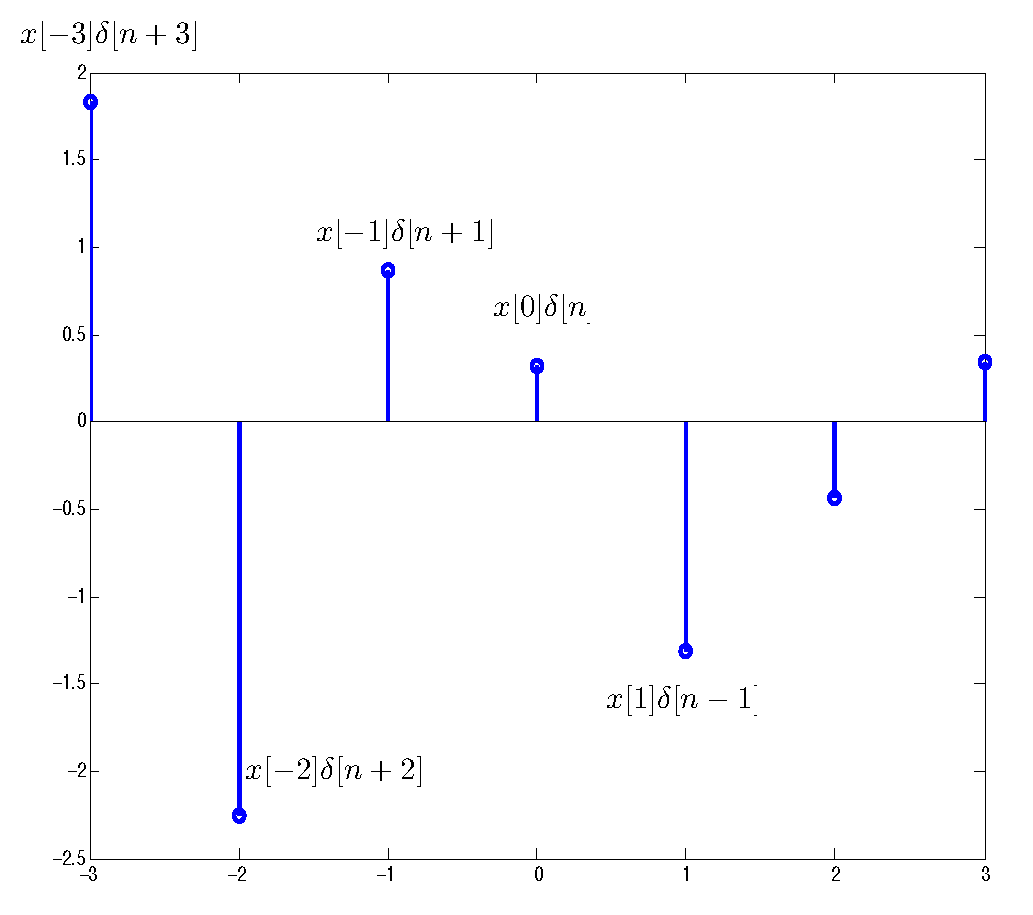
\includegraphics[scale=0.35]{Figures/Signal64.pdf}
%\end{figure}
%}
%
%\frame{
%\frametitle{Unit Step Sequence}
%
% \begin{align}\nn
%u[n]=\left\{
%\begin{array}{cc}
%1 & n\geq0\\
%0 & n< 0
%\end{array}
%\right.
%\end{align}
%
%\begin{block}{From $\delta[n]$ to $u[n]$}
%As we have seen, we can decompose it as a sum of unit impulse sequences:
%\begin{align}\nn
%u[n]&=\sum_{k=-\infty}^{\infty}u[k]\delta[n-k]=\sum_{0}^{\infty}\delta[n-k]\\\nn
%u[n-n_0]&=\sum_{k=-\infty}^{\infty}u[k-n_0]\delta[n-k]=\sum_{n_0}^{\infty}\delta[n-k]
%\end{align}
%\end{block}
%}
%
%\frame{
%\frametitle{Unit Step Sequence}
%
%\begin{block}{From $u[n]$ to $\delta[n]$}
%
%We can also obtain $\delta[n]$ from $u[n]$:
%
%\begin{align}\nn
%\delta[n]&=u[n]-u[n-1]\\\nn
%\delta[n-n_0]&=u[n-n_0]-u[n-n_0-1]
%\end{align}
%\end{block}
%
%
%}
%
%\subsection{Continuous-time Unit Step and Unit Impulse}
%
%\frame{
%\frametitle{Unit Step signal}
%Similar to the discrete case:
%\begin{align}
%\nn
%u(t)=\left\{
%\begin{array}{cc}
%1 & t\geq0\\
%0 & t< 0
%\end{array}
%\right.
%\end{align}
%
%\begin{block}{Continuous approximation}
%Let 
%\begin{align}
%\nn
%u_L(t)=\left\{
%\begin{array}{cc}
%0 & t<0\\
%t/L & 0<t<L\\
%1 & t\geq L
%\end{array}
%\right.
%\end{align}
%then
%\begin{align}\nn
%\lim_{L\rightarrow 0}u_L(t)=u(t)
%\end{align}
%\end{block}
%
%
%}
%
%
%%\frame{
%%\frametitle{Rectangular pulse}
%%
%%\begin{align}
%%\nn
%%\Pi(t)=\left\{
%%\begin{array}{cc}
%%1 & |t|\leq\frac{1}{2}\\
%%0 & \text{otherwise}
%%\end{array}
%%\right.
%%\end{align}
%%
%%In general:
%%\begin{align}
%%\nn
%%\Pi\left(\frac{t-a}{b}\right)=\left\{
%%\begin{array}{cc}
%%1 & |t-a|\leq\frac{b}{2}\\
%%0 & \text{otherwise}
%%\end{array}
%%\right.
%%\end{align}
%%
%%\begin{figure}
%%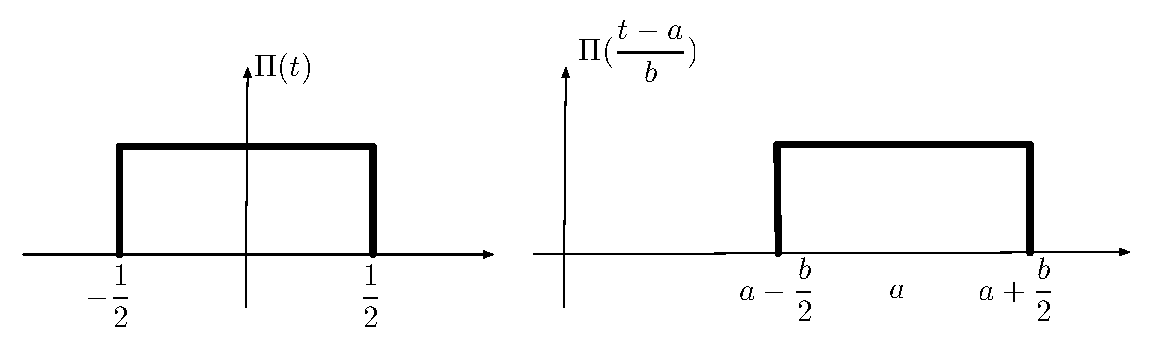
\includegraphics[scale=0.6]{Figures/Signal65.pdf}
%%\end{figure}
%%
%%}
%%
%%\frame{
%%\frametitle{Rectangular pulse}
%%
%%It can be defined in terms of the unit step signal $u(t)$:
%%\begin{align}\nn
%%\Pi(t)&=u(t+\frac{1}{2})-u(t-\frac{1}{2})\\\nn
%%\Pi(\frac{t-a}{b})&=u(t-(a-\frac{b}{2}))-u(t-(a+\frac{b}{2}))
%%\end{align}
%%
%%
%%}
%
%\frame{
%\frametitle{Continuous-time impulse (Dirac Delta function)}
%
%The continuous-time impulse function $\delta(t)$ is related to the unit step by the equation
%\begin{align*}
%u(t)=\int_{-\infty}^{t}\delta(\tau)d\tau
%\end{align*}
%and this suggests that
%\begin{align}\nn
%\delta(t)=\frac{\partial u(t)}{\partial t}=\left\{
%\begin{array}{cc}
%\infty & t=0\\
%0 & t\neq0
%\end{array}
%\right.
%\end{align}
%
%\begin{figure}
%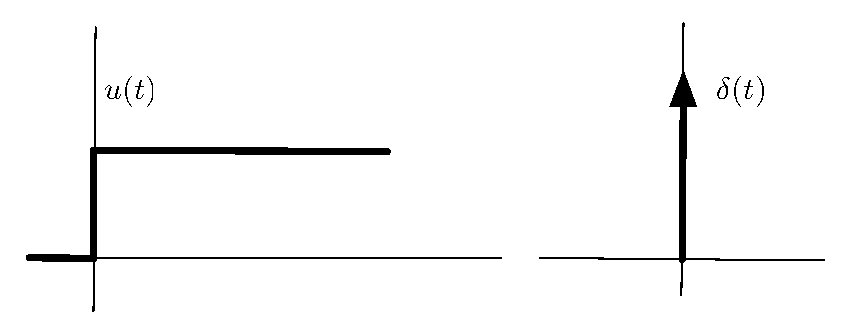
\includegraphics[scale=0.6]{Figures/Signal66.pdf}
%\end{figure}
%
%}
%
%\frame{
%\frametitle{Continuous-time impulse (Dirac Delta function)}
%
%\begin{block}{Continuous approximation}
%Let 
%\begin{align}
%\nn
%\delta_L(t)=\frac{\partial u_L(t)}{\partial t}\left\{
%\begin{array}{cc}
%L^{-1} & 0<t<L\\
%0 & \text{ otherwise }
%\end{array}
%\right.
%\end{align}
%then
%\begin{align}\nn
%\delta(t)=\lim_{L\rightarrow 0}\delta_L(t)
%\end{align}
%\end{block}
%
%\begin{figure}
%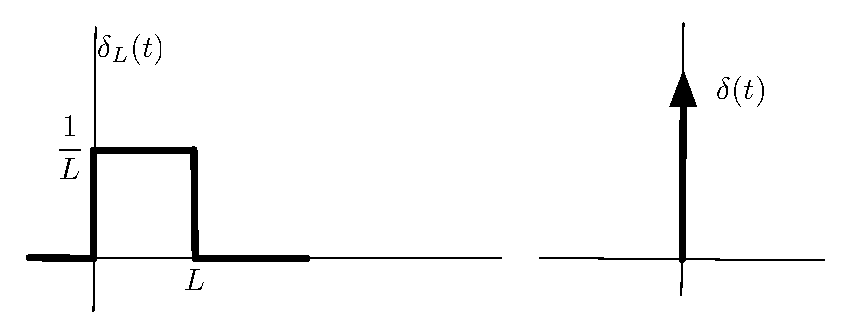
\includegraphics[scale=0.5]{Figures/Signal67.pdf}
%\end{figure}
%
%}
%
%\frame{
%For any $L$ value,
%\begin{align}\nn
%&\int_{-\infty}^{\infty}\delta_L(t) dt=L\frac{1}{L}=1 \Rightarrow  \int_{-\infty}^{\infty} \delta(t)=1.
%\end{align}
%
%\begin{exampleblock}{}
%The signal $\delta(t)$ has unit area.
%\end{exampleblock}
%
%\begin{block}{}
%\begin{align}\nn
%\int_{-\infty}^{\infty}\delta(t-t_0)dt=1
%\end{align}
%\end{block}
%
%}
%
%\frame{
%\frametitle{Continuous-time Impulse. Properties.}
%
%\begin{block}{Multiplication by a constant $\rightarrow$ Area multiplication}
%\begin{align}\nn
%\int_{-\infty}^{\infty}k\delta(t)dt=k\int_{-\infty}^{\infty}\delta(t)dt=k
%\end{align}
%\end{block}
%
%\begin{exampleblock}{$x(t)\delta(t-t_0)$}
%\begin{align}\nn
%x(t)\delta(t-t_0)=x(t_0)\delta(t-t_0)
%\end{align}
%\end{exampleblock}
%
%\begin{figure}
%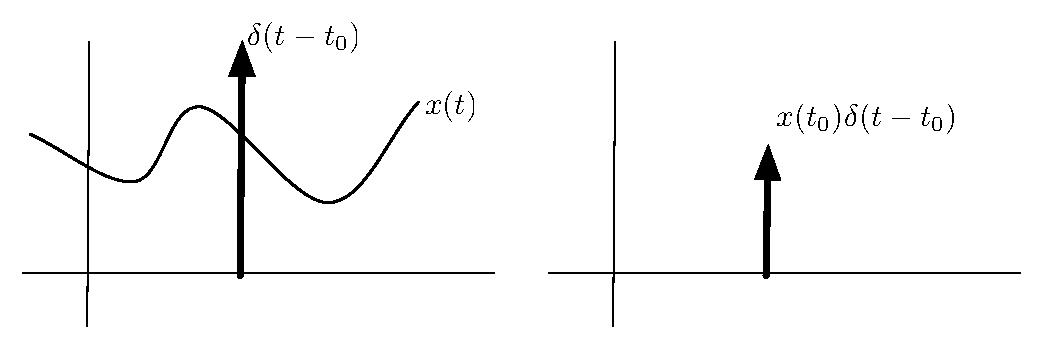
\includegraphics[scale=0.5]{Figures/Signal68.pdf}
%\end{figure}
%
%}
%
%\frame{
%\frametitle{Continuous-time Impulse. Properties (II).}
%
%Any signal $x(t)$ can be decomposed as a linear combination of an infinite number of impulses:
%\begin{align}\nn
%x(t)=\int_{-\infty}^{\infty}x(\tau)\delta(t-\tau) d\tau
%\end{align}
%
%\begin{exampleblock}{Unit step signal}
%\begin{align}\nn
%u(t)=\int_{-\infty}^{\infty}u(\tau)\delta(t-\tau) d\tau=\int_{0}^{\infty}\delta(t-\tau) d\tau
%\end{align}
%\end{exampleblock}
%
%}
%
%%\frame{
%%\frametitle{Relationship with the rectangular pulse}
%%
%%\begin{figure}
%%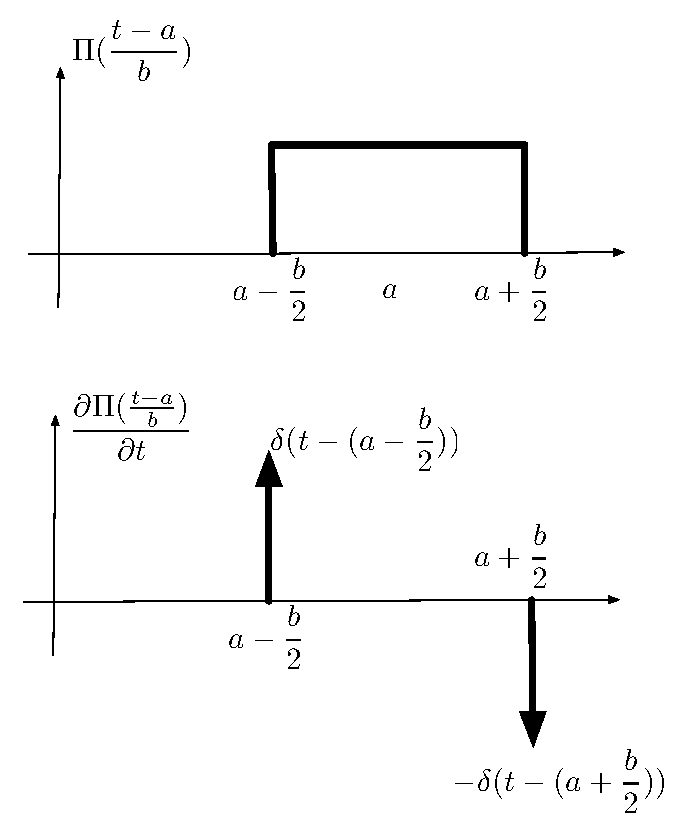
\includegraphics[scale=0.5]{Figures/Signal69.pdf}
%%\end{figure}
%%
%%}


\end{document}
